\section{Problema 4}

\subsection*{Problema 4}
Implementa el algoritmo Spline Natural Cúbico y realiza la interpolación para la ecuación \ref{eq:problema4a} a partir de los siguientes puntos de las ecuaciones \ref{eq:x_points} y \ref{eq:y_points}.
\begin{equation}
	f(x) = \frac{x}{1+x^2} \label{eq:problema4a}
\end{equation}

\begin{align}
	x & = \frac{i-8}{2} \qquad i=0,1,2,\dots,16 \label{eq:x_points} \\
	y & = f(x) \label{eq:y_points}
\end{align}
\begin{figure}[H]
	\centering
	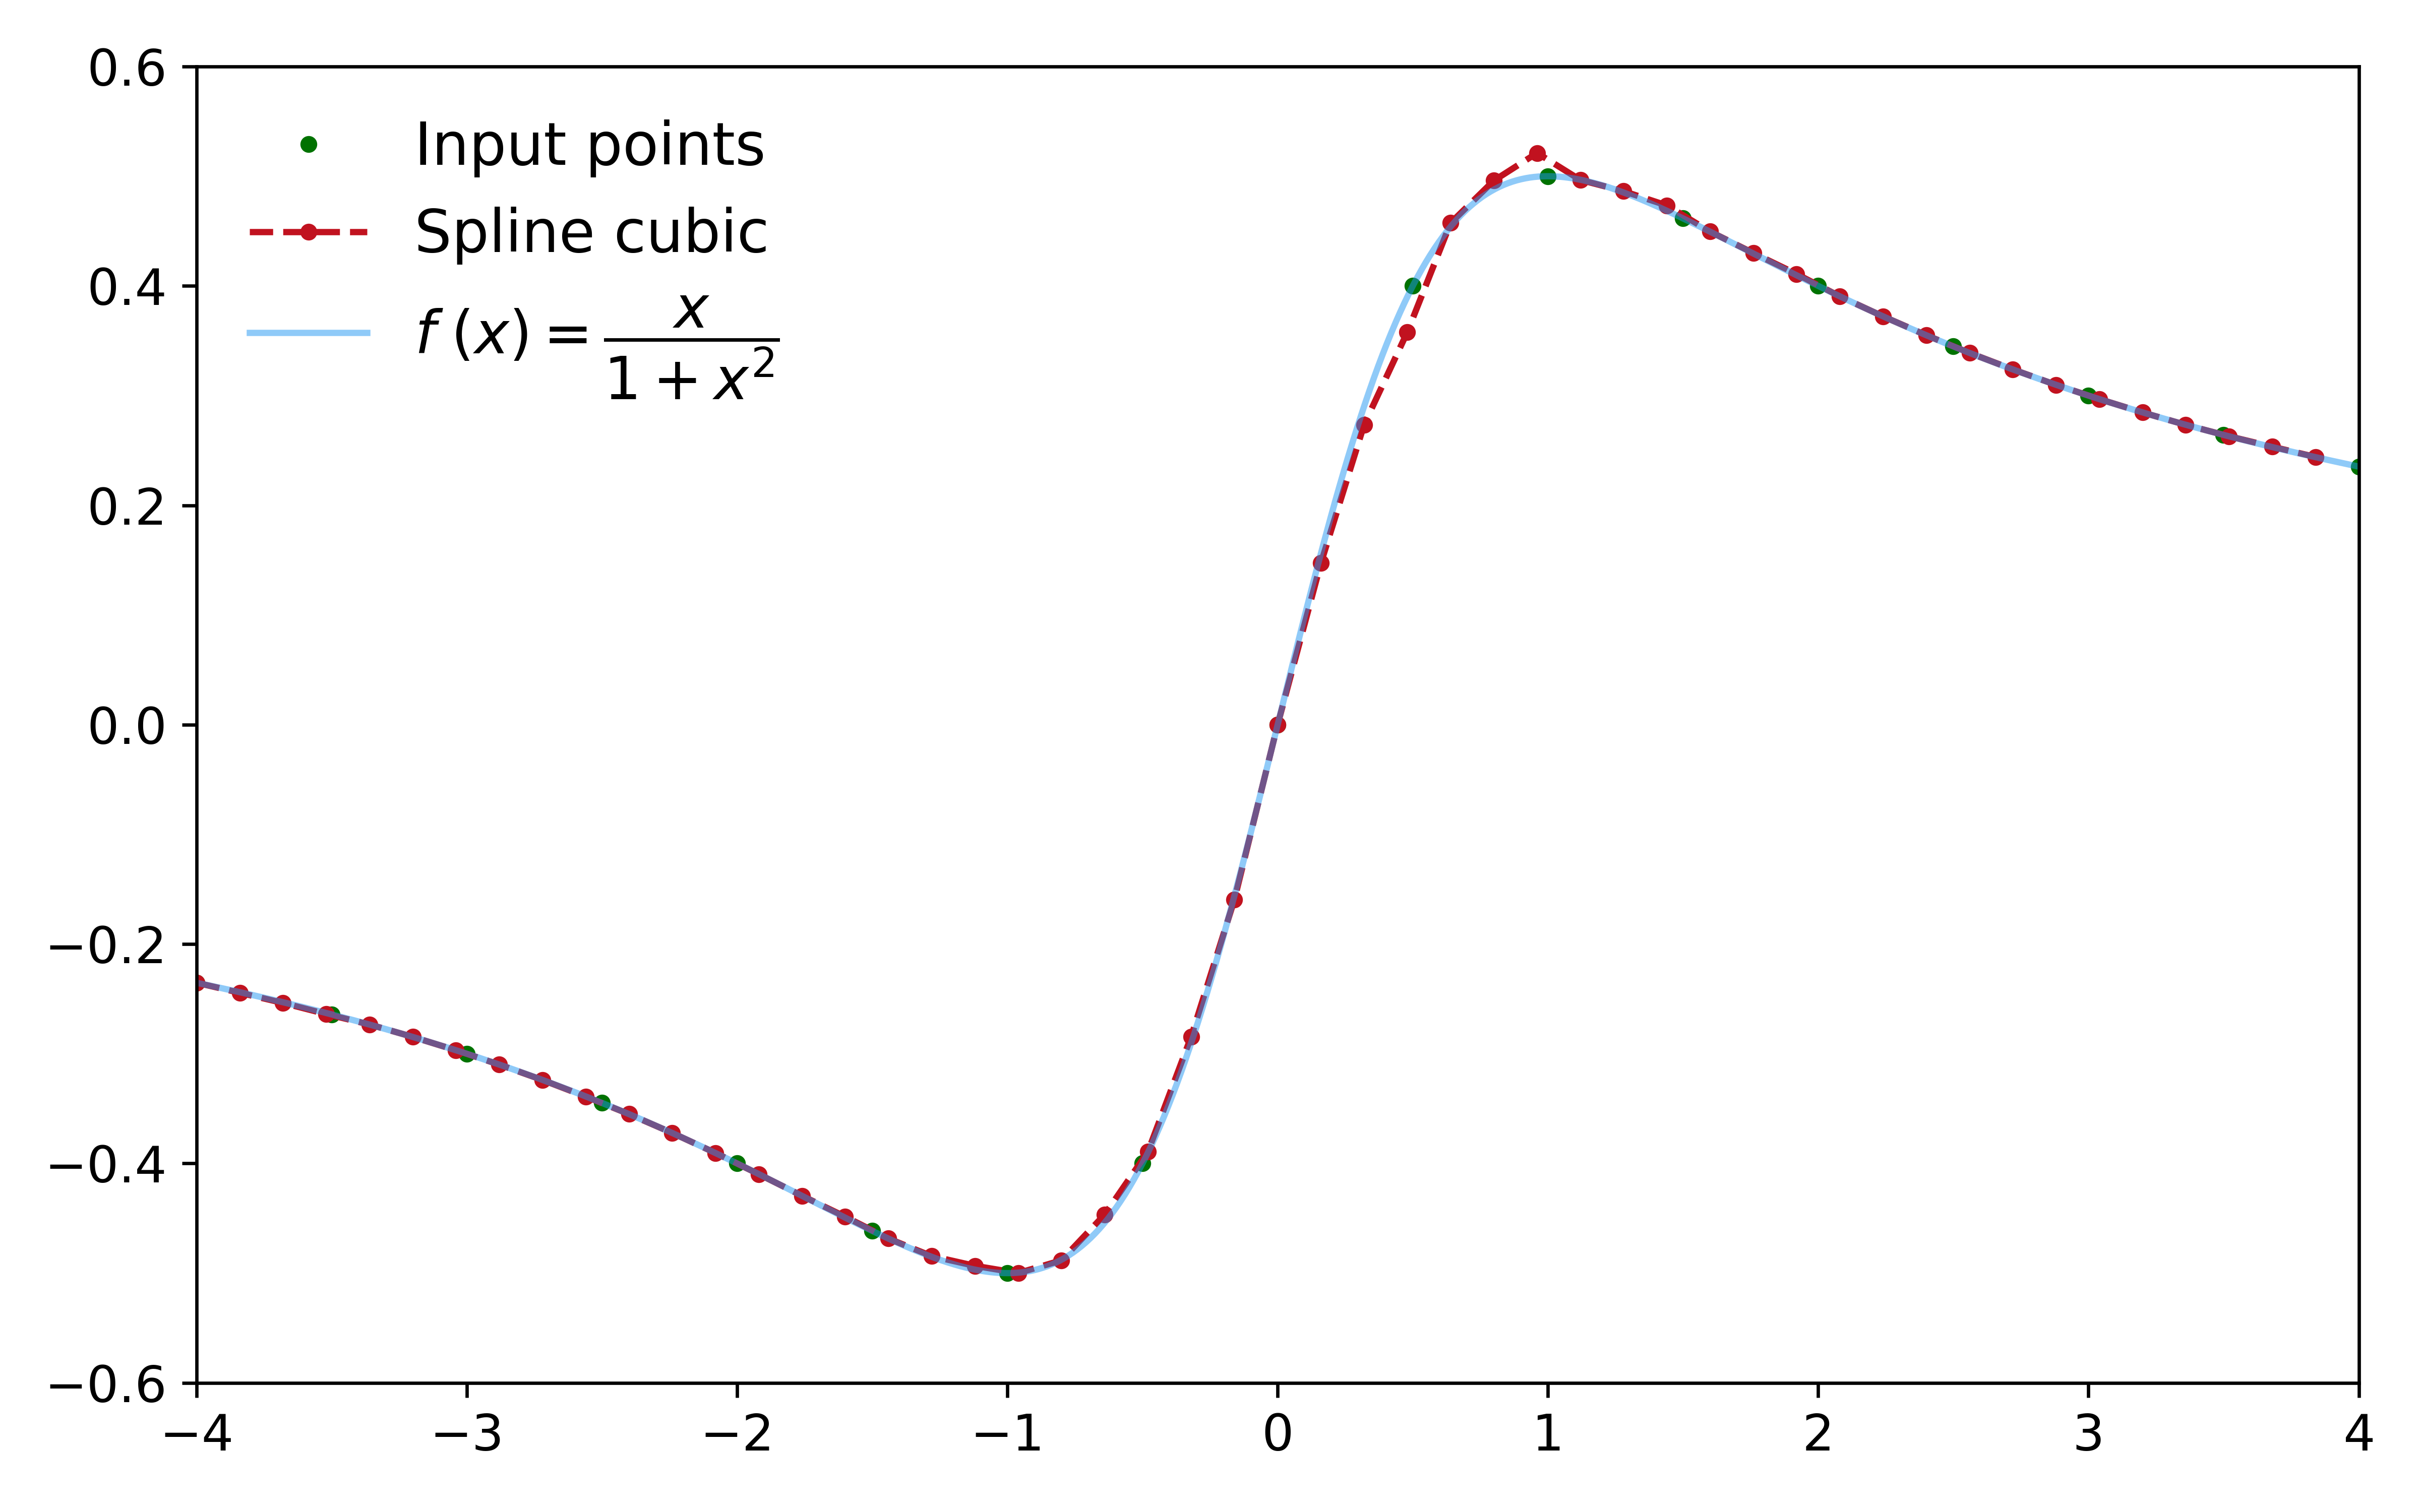
\includegraphics[width=14cm]{Graphics/problema04a.png}
	\caption{Interpolación de la ecuación \ref{eq:problema4a} dados los puntos generados con las ecuaciones \ref{eq:x_points} y \ref{eq:y_points}.}
\end{figure}
